\documentclass[a4paper,12pt]{article} % тип документа

%  Русский язык
\usepackage[T2A]{fontenc}			% кодировка
\usepackage[utf8]{inputenc}			% кодировка исходного текста
\usepackage[english,russian]{babel}	% локализация и переносы

\usepackage{graphicx}               % импорт изображений
\usepackage{wrapfig}                % обтекаемые изображения
\graphicspath{{pictures/}}          % обращение к подкаталогу с изображениями
\usepackage[14pt]{extsizes}         % для того чтобы задать нестандартный 14-ый размер шрифта
\usepackage{amsfonts}               % буквы с двойными штрихами
\usepackage[warn]{mathtext}         % русский язык в формулах
\usepackage{indentfirst}            % indent first
\usepackage[margin = 25mm]{geometry}% отступы полей
\usepackage{amsmath}                % можно выводить фигурные скобочки -- делать системы уравнений
\usepackage[table,xcdraw]{xcolor}   % таблицы
\usepackage{amsmath,amsfonts,amssymb,amsthm,mathtools} % Математика
\usepackage{wasysym}                % ???
\usepackage{upgreek}                % ???  
\usepackage{caption}
\usepackage{multirow}
\captionsetup{labelsep=period}
\usepackage{gensymb} % degree symbol


\begin{document}
	
	
	\begin{center}
		
		
		\textbf{НАЦИОНАЛЬНЫЙ ИССЛЕДОВАТЕЛЬСКИЙ УНИВЕРСИТЕТ \\ <<МОСКОВСКИЙ ФИЗИКО-ТЕХНИЧЕСКИЙ ИНСТИТУТ>>}
		\vspace{13ex}
		
		\textbf{Лабораторная работа 4.4.3\\ <<Изучение призмы с помощью гониометра>>}
		\vspace{40ex}
		
		\normalsize{Овсянников Михаил Александрович \\ студент группы Б01-001\\ 2 курс ФРКТ\\}
	\end{center}
	
	\vfill 
	
	\begin{center}
		г. Долгопрудный\\ 
		2022 г.
	\end{center}
	
	
	\thispagestyle{empty} % выключаем отображение номера для этой страницы
	\newpage
	
	
	\textbf{Цель работы:} Знакомство с работой гониометра, исследование дисперсии стеклянной призмы и определение характеристик призмы как спектрального прибора.
	
	
	\textbf{В работе используются:} гониометр, ртутная лампа, призма, стеклянная плоскопараллельная пластинка, призменный уголковый отражатель.
	
	\section*{Теоретические сведения}
	Гониометр служит для точного измерения углов и находит широкое применение в оптических лабораториях. С помощью гониометра можно определять показатели преломления и преломляющие углы призм и кристаллов, исследовать параметры дифракционных решёток, измерять длины волн спектральных линий и т. д. В настоящей работе прибор применяется для исследования дисперсии стеклянных призм — зависимости показателя преломления от длины волны.
	
	Угол минимального отклонения $\delta$, преломляющий угол $\alpha$ и показатель преломления $n$ связаны между собой соотношением:
	\begin{equation*}
		n = \frac{\sin{\frac{\alpha + \delta}{2}}}{\sin{\frac{\alpha}{2}}}
	\end{equation*}

	Измерив с помощью гониометра преломляющий угол призмы и углы наименьшего отклонения для света разных длин волн, можно рассчитать величину $n$ и построить дисперсионную кривую — график зависимости $n(\lambda)$.
	
	По дисперсионной кривой могут быть определены такие важные характеристики оптических стёкол, как средняя дисперсия:
	\begin{equation*}
		D = n_F - n_C
	\end{equation*}

	и коэффициент дисперсии $\nu$:
	\begin{equation*}
		\nu = \frac{n_D - 1}{n_F - n_C}
	\end{equation*}

	Здесь $n_D$, $n_F$ и $n_C$ — показатели преломления для $\lambda_D$ = 589,3 нм (среднее значение длин волн жёлтого дублета натрия), $\lambda_F$ = 486,1 нм (голубая линия водорода), $\lambda_C$ = 656,3 нм (красная линия водорода).
	
	\newpage
	
	По наклону дисперсионной кривой можно оценить разрешающую способность призмы:
	\begin{equation*}
		R = \frac{\lambda}{\delta \lambda} = b\frac{dn}{d\lambda}
	\end{equation*}
	
	\section*{Экспериментальная установка}
	
	\begin{figure}[h!]
		\centering
		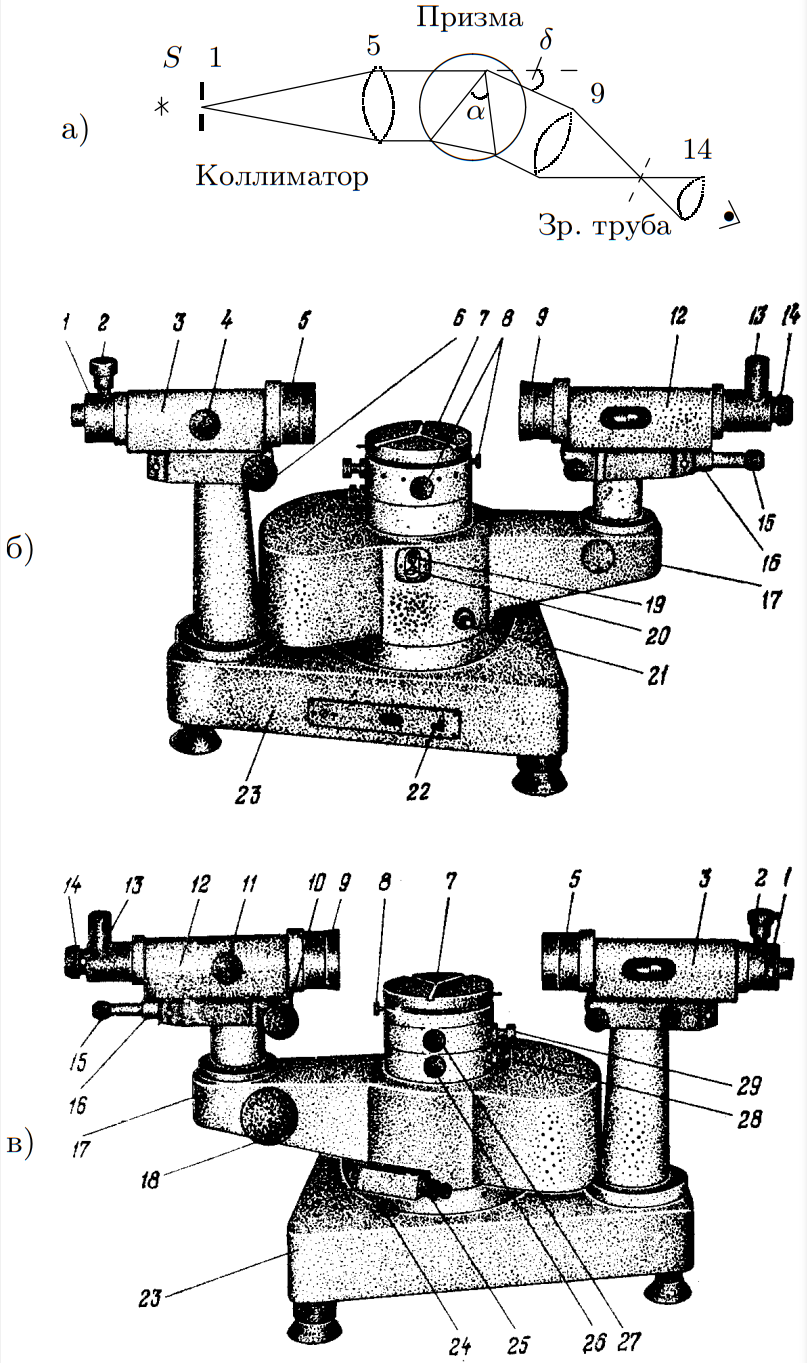
\includegraphics[scale=0.65]{Pictures/Установка}
		\caption{Гониометр}
	\end{figure}

	Оптическая схема гониометра представлена на рис. 1а. Свет от источника $S$ проходит через коллиматор и преобразуется призмой или решёткой в набор параллельных пучков, каждый из которых соответствует определённой длине волны. Параллельные пучки собираются в фокальной плоскости объектива 9 зрительной трубы и рассматриваются глазом через окуляр 14.
	
	Внешний вид гониометра представлен на рис. 1б и 1в. Коллиматор 3, столик 7 и алидада 17 со зрительной трубой 12 крепятся на массивном основании 23. На столике 7 размещаются исследуемые объекты. Коллиматор закреплён неподвижно, а столик и алидада с трубой могут вращаться вокруг вертикальной оси.
	
	Важнейшим узлом гониометра является устройство, служащее для отсчёта угла поворота зрительной трубы вокруг вертикальной оси, проходящей через центр столика. На этой оси крепится прозрачное кольцо (лимб), расположенное в корпусе прибора. На поверхности лимба нанесена шкала с делениями. На поверхности лимба нанесена шкала с делениями. Лимб разделён на $3 \times 360 = 1080$ делений. Цена деления 200, оцифровка делений произведена через $1^\circ$. Шкалу лимба можно наблюдать через окуляр отсчётного устройства 16 при включённой подсветке (тумблер 22). Резкость изображения шкалы регулируется вращением оправы окуляра 15.
	
	Оптическая система отсчётного устройства собрана так, что через окуляр можно наблюдать изображения штрихов двух диаметрально противоположных участков лимба, причём одно изображение прямое, а другое обратное. Кроме того, оптическая система позволяет перемещать эти изображения друг относительно друга, оставляя в покое как лимб, так и алидаду со зрительной трубой.
	
	\vspace{40mm}
	В работе предлагается отъюстировать гониометр, определить преломляющий угол призмы, измерить углы наименьшего отклонения для нескольких спектральных линий ртути и оценить спектральные характеристики призмы.
	
	\newpage
	
	\section*{Ход работы}
	
	\begin{center}
		\textbf{I. Юстировка гониометра}
	\end{center}

	\begin{enumerate}
	\item Для начала установим зрительную трубу на бесконечность
	\item Затем отрегулируем поверхность столика перпендикулярно оси вращения прибора 
	\item После произведем настройку коллиматора
	\item И, в конце концов, установим начало отсчёта.
	\end{enumerate}

	\begin{center}
		\textbf{II. Установка призмы}
	\end{center}

	Поставим рабочую призму так, чтобы её преломляющее ребро было вертикально, а одна из рабочих граней была перпендикулярна одному из установочных винтов 8.
	
	Установим рабочую грань призмы перепендикулярно второму из винтов 8 и найдем отраженный крест.

	\begin{center}
		\textbf{III. Измерение преломляющего угла}
	\end{center}

	Для измерения преломляющего угла призмы установим трубу перпендикулярно одной из её отражающих граней и снимем отсчёт по лимбу. Затем, не трогая призму и столик, повернем алидаду с трубой вокруг преломляющего угла призмы и проведем ту же операцию для другой рабочей грани. По углу поворота трубы рассчитаем преломляющий угол призмы:
	\begin{equation*}
		\alpha = 59^\circ 18'27''.
	\end{equation*}

	\begin{center}
		\textbf{IV. Минимальный угол отклонения}
	\end{center}

	Для определения минимального угла отклонения $\delta$ поставим призму на столике так, чтобы её основание было параллельно оси коллиматора. Расположим лист бумаги за призмой и найдем на нём спектр, вращая столик рукой. Продолжая поворачивать столик и наблюдая за перемещением спектра, найдем положение столика с призмой, соответствующее минимальному отклонению преломленного луча от направления падающего луча. Измеренные значения углов $\delta$ запишем в таблицу 1:
	
	\newpage
	
	\begin{table}[h!]
		\centering
		\resizebox{\columnwidth}{!}{%
		\begin{tabular}{|c|c|c|c|c|c|c|c|c|}
			\hline
			Линия         & $K_1$              & $K_2$              & 1                 & 2                 & 3                  & 4                 & 5                  & 6                  \\ \hline
			Цвет          & красн              & красн              & желт              & желт              & зелен              & голуб             & синий              & фиол               \\ \hline
			Угол $\delta$ & $51^\circ 12'38''$ & $51^\circ 38'52''$ & $52^\circ 1'23''$ & $52^\circ 2'42''$ & $52^\circ 22'30''$ & $53^\circ 6'45''$ & $54^\circ 18'29''$ & $55^\circ 18'40''$ \\ \hline
		\end{tabular}%
	}
	\caption{Минимальные углы отклонения для линий}
	\end{table}

	
	\begin{center}
		\textbf{V. Разрешающая способность}
	\end{center}

	Для оценки разрешающей способности призмы измерим угловую ширину одной из желтых линий дублета, предварительно установив минимально возможную ширину входной щели: $\Delta \delta = 39''$. 
	
	Измерим линейкой длину основания призмы: $b = (7,5 \pm 0,1)$ см.
	
	
	\begin{center}
		\textbf{VI. Обработка результатов}
	\end{center}

	1) Рассчитаем показатель преломления $n(\alpha, \delta)$. Результаты заносим в таблицу 2:
	
	\begin{table}[h!]
		\centering
		\resizebox{\columnwidth}{!}{%
		\begin{tabular}{|c|c|c|c|c|c|c|c|c|}
			\hline
			$\lambda$, нм & 690,7              & 623,4              & 579,1             & 577,0             & 546,1              & 491,6             & 435,8              & 404,7              \\ \hline
			$\delta$      & $51^\circ 12'38''$ & $51^\circ 38'52''$ & $52^\circ 1'23''$ & $52^\circ 2'42''$ & $52^\circ 22'30''$ & $53^\circ 6'45''$ & $54^\circ 18'29''$ & $55^\circ 18'40''$ \\ \hline
			$n$          & 1,6609             & 1,6653             & 1,6690            & 1,6692            & 1,6725             & 1,6798            & 1,6914             & 1,7010             \\ \hline
		\end{tabular}%
	}
	\caption{Зависимость $n(\delta)$, или $n(\lambda)$}
	\end{table}

	Теперь построим дисперсионную кривую $n(\lambda)$.
	\begin{figure}[h!]
		\centering
		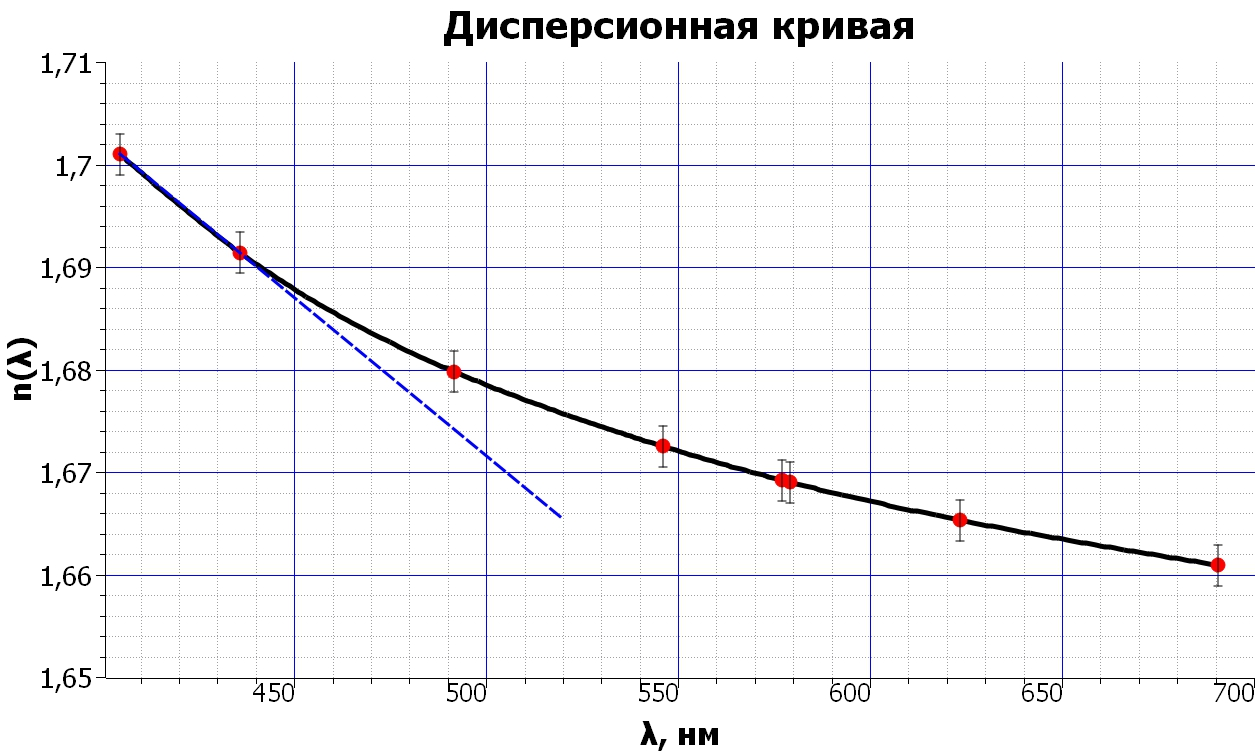
\includegraphics[scale=0.55]{Pictures/Кривая}
		\caption{Дисперсионная кривая}
	\end{figure}
	
	Погрешность $\sigma_n = 0,002$ везде.

	2) Определим по графику $n_D$, $n_F$ и $n_C$. Получаем значения:
	
	\begin{equation*}
		n_D = (1,668 \pm 0,002) \hspace{10mm} n_F = (1,682 \pm 0,002) \hspace{10mm} n_C = (1,663 \pm 0,002) 
	\end{equation*}

	Теперь рассчитаем среднюю дисперсию $D = n_F - n_C$:
	\begin{equation*}
		\boxed{D = (0,019 \pm 0,003)}
	\end{equation*}

	И число Аббе $\nu = \dfrac{n_D - 1}{n_F - n_C} = \dfrac{n_D - 1}{D}$:
	\begin{equation*}
		\boxed{\nu = (35 \pm 6)}
	\end{equation*}

	Определим по таблицам сорт стекла.
	\begin{figure}[h!]
		\centering
		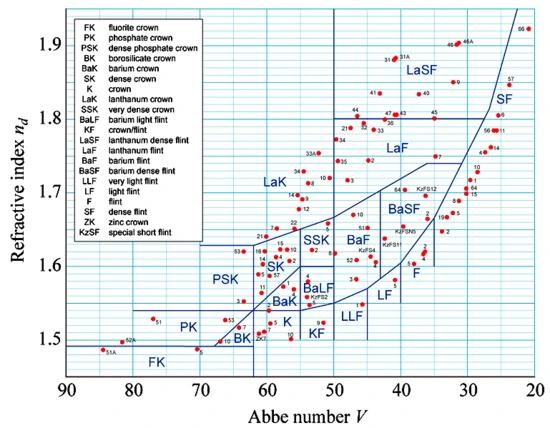
\includegraphics[scale=1.2]{Pictures/Стекло}
		\caption{Диаграмма Аббе}
	\end{figure}

	Из диаграммы видно, что в данном эксперименте стекло из сорта баритового флинта.
	
	\newpage
	
	3) По наклону кривой $dn/d\lambda$ рассчитаем максимальную разрешающую способность призмы:
	\begin{equation*}
		R = b\frac{dn}{d\lambda}.
	\end{equation*}	
	
	Из графика получаем, что:
	\begin{equation*}
		\left(\frac{dn}{d\lambda}\right)_{\text{max}} = (31 \pm 5) \cdot 10^{-5} \text{ нм}^{-1} = (31 \pm 5) \cdot 10^2 \text{ см}^{-1}.
	\end{equation*}

	Тогда максимальная разрешающая способность:
	\begin{equation*}
		\boxed{R = (23250 \pm 3800)}
	\end{equation*}

	Рассчитаем экспериментальную величину $R$ по измерениям желтого дублета:
	\begin{equation*}
		\boxed{R = \frac{\lambda}{\delta \lambda} = 560}
	\end{equation*}

	Оценим, при каком размере решетки, имеющей $d^{-1} = 100$ штр/мм, она обладает такой же разрешающей способностью в первом порядке, как призма с основанием $b = 5$ см:
	\begin{equation*}
		a\cdot 100 = b\frac{dn}{d\lambda}
	\end{equation*}
	Откуда получаем $a = (155 \pm 25)$ мм.
	
	4) Рассчитаем угловую дисперсию $d\varphi/d\lambda$ по измерениям желтого дублета:
	\begin{equation*}
		\frac{d\varphi}{d\lambda} = \frac{\delta_{\text{желт}_1} - \delta_{\text{желт}_2}}{\lambda_{\text{желт}_1} - \lambda_{\text{желт}_2}}
	\end{equation*}

	Получаем следующее значение:
	\begin{equation*}
		\boxed{\frac{d \varphi}{d \lambda} = (182 \pm 3) \cdot 10^{-6} \; \frac{\text{рад}}{\text{нм}} = (182 \pm 3) \text{ мм}^{-1}}
	\end{equation*}

	И теперь сравним её с дисперсией решетки в первом порядке, имеющей $d^{-1} = 100$ штр/мм:
	\begin{equation*}
		\boxed{\frac{d \varphi}{d \lambda} \approx \frac{1}{d} = 100 \text{ мм}^{-1}}
	\end{equation*}
	
	Как видим, дисперсия, измеренная по дублету, и дисперсия решетки имеют одинаковый порядок, однако у дублета она в $\thicksim 2$ раза больше. 
	
	\newpage
	
	\section*{Вывод}
	Самым главным в этой работе стало знакомство с работой гониометра. В дополнение к этому мы провели исследование дисперсии стеклянной призмы и определили характеристики призмы как спектрального прибора:
	\begin{equation*}
		n_D = (1,668 \pm 0,002) \hspace{10mm} n_F = (1,682 \pm 0,002) \hspace{10mm} n_C = (1,663 \pm 0,002);
	\end{equation*}

\noindent	Средняя дисперсия:
	
\noindent	$D = (0,019 \pm 0,003)$;

\noindent	Число Аббе:
	
\noindent	$\nu = (35 \pm 6)$;

\noindent	Экспериментальная разрешающая способность:
	
\noindent	$R = 560$;
	
\noindent	Угловая дисперсия:
	
\noindent	$\frac{d \varphi}{d \lambda} = (182 \pm 3) \text{ мм}^{-1}$.

\vspace{5mm}

	Как видно, ошибки небольшие и максимальная составляет $\thicksim 17\%$. Все эти ошибки связаны с неточностью измерений и несовершенством техники ее проведения.

\end{document}